% Chapter 3

\chapter{Problem Description}
\label{Chapter3}
\lhead{Chapter 3. \emph{Problem Description}}

\section{Reproducible research}
New scientific ideas, developments and results are only useful when
they are documented and published. It is vital that results are
announced, so others can be aware of the latest developments on their
field of research. This helps in creating a linked data cloud, used by
scientists to incorporate various output of other research into their
own, using previous results as "stepping stones" to achieve something
new.\cite{babbccrddg10} But simply publishing results is not enough in
order for others to make use of them. Besides announcing the
achievements, the other goal of scientific publications is to convince
the readers that the results it presents are correct. Besides
theoretical reasoning, papers in experimental science should provide a
documented methodology describing how the author has gotten to those
results.\cite{m10} The methodology has to be detailed and precise
enough so other researchers can repeat the same steps, thus
reproducing the same results. This is vital in order to provide the
possibility to verify those results and to fully understand
them. Reproducing the results also makes for a starting point for
further development, as the described methods used for reproduction
can be extended to achieve something more or something different in
the same area of research, or repurposed to gain useful results in a
completely different area. This subject is relevant to SMPI and one of
the main goals of the testing and validation framework is to make
developments in the area.
\section{Testing framework}
SMPI is an actively developed project and as such, a lot of tests are
run and a lot of measurements are taken. Previous papers
(\cite{csgscq11} \cite{bdglmqssv13}) have shown, amongst other
results, how accurate the performance predictions SMPI makes are and
how the time of the simulation can be lowered, while getting very
little differences in simulated time (which means the predicted
performance). These results are obtained through extensive testing and
as development continues, more and more test data is needed for
verification purposes. In order to get results, both
real-life (RL) tests and on-line simulation tests using SimGrid (SG)
are needed to be obtained and then the results need to be visualized,
analyzed and compared. Comparison is very important, since this is how
we can validate SMPI. All this needs to be done in as many different
kinds of environments as possible. Currently, this is a tedious task
that needs a lot of configuration by hand, as there is no unified
methodology or automation for setting up experiments and obtaining
results on
different kinds of distributed environments and for different kinds of
MPI implementations - one has to find his/her own way to make it
work. Documentation only exists for specific systems, for example in
\cite{ms11}, there is a guide about how to produce time-independent RL
traces on the Grid'5000 testbed. Obviously, platform-specific guides
don't always help with problems arising in an other environment.\\
Below comes a more detailed description of the process of acquiring
traces.
\section{Obtaining traces}
\subsection{On-line SG traces}
In order to conduct tests on the simulator, the first step is to
create the simulated environment. This is done by creating a platform
file that can be fine-tuned to model the desired system. \#maybe
detail how a platform file looks like?\#
\subsection{RL traces}
As talked about in detail in \cite{ms11}, conducting RL tests involves
multiple steps. RL test data collection is done by collecting traces
of MPI benchmarks. Currently, the favored tool in trace collection in
the project is Tuning and Analisys Utilities (TAU)\cite{sm06}, which
is a well-established profiling tool, that also provides tracing
features. Thus, on the system
where we are running the benchmarks, TAU has to be deployed and
configured, alongside other software that TAU depends on. One is
PAPI\cite{mbdh99}\cite{lmmsl01},
an interface which provides us with the possibility to
get access to low-level hardware counters (to trace the number of
instructions at processor level). We also need the Program Database
Toolkit (PDT)\cite{lcmsmrr00}, which provides the ability of automatic performance
instrumentation. In order for TAU to collect the traces we need, these
toolkits have to be deployed and correctly linked with TAU. TAU has
its own compiler scripts for MPI programs for both Fortran, C and
C++. After compiling a benchmark using one of these scripts, they will
generate TAU trace files upon execution. One trace file (.trc)
and one event file (.edf) is generated for each MPI process.\\
It is possible to visualize the traces, in order to compare the RL and SG
results more easily. Paje is a visualization tool that can be used for
this purpose. It has its own trace format that it can comprehend, thus
the TAU traces have to be converted to that. Also, we need to merge
the traces into one file that we can give to Paje after the
conversion. There is a
TAU script that is able to do this, creating one trace and one event
file. We now only have the task of converting the TAU trace to a Paje
trace file. Another MPI tracing library, Akypuera provides this
possibility, having its own tau-to-paje conversion script. Once done,
we finally have a trace file that Paje can read and display to us.\\
In the future, it is very likely that more and more tests will have to
be run in order to verify old and newly implemented features, as well
as various experiments will be conducted using SMPI to test it against
various MPI platforms. The main reason of importance of developing an
automated way for testing and validation is that it could make the
previously discussed tedious trace-gathering process a lot smoother
and faster, with less user interaction. If the process could be
incorporated into a single workflow, that would make it much easier
for the user to procure test results. This way, proportionally more
tests could be run, providing more reliable results with less effort
than before. Apart from making extensive testing and experimentation
more straightforward, a functioning test and
validation framework would provide a well-documented method, which
could be used by other researchers to reproduce the achieved results,
the importance of which is discussed above.
\section{Tracing-related problems}
Apart from wanting to simplify the previously described, fairly
convoluted process of getting results, there are other problems
related to tracing that need to be addressed. Since we need to compare
RL and SG traces, it is very important that the traces we get are
accurate, otherwise we could be lead to false conclusions. Below are
the most prominent traps that could potentially compromise our
results. Note that these are problems that come up in a real
environment, thus only related to real-life traces.
\subsection{Multiple cores on one node}
Nowadays, it is common for a computer to have multiple processors
(cores). Because of this, applications have been optimized to increase
performance by utilizing more than one core. MPI implementations have
also been optimized to migrate threads between cores in certain
cases. The problem with this is that SMPI is not configured to account
for the speedup that the utilization of multi-core processors can
cause. So if we compare the running time of an MPI application that
was run on multi-core nodes and compare the running time to our
simulation's running time that was done by using SMPI, even if we
simulated the used platform correctly, we will likely see that SMPI
overestimated the running time, since it didn't take into account the
performance increase caused by using multiple cores.\\
A solution to this problem is to explicitly disable all cores but one
on every node before running the real-life experiment.\cite{ms11}
The downsides to doing this are that we need to know the
platform-specific
instructions on the nodes which have to be given to disable cores, as
well as we most likely need root privileges. But if we can use it,
this method is a simplistic and sure way to solve this problem.\\
Another possible way to make sure that MPI doesn't make use of having
multiple cores at its disposal is to specifically bind MPI processes
to cores. For example for OpenMPI 1.4 and above, this can be done by
using the processor affinity instruction parameter
\emph{-{}-bind-to-core} when running the application.
\subsection{Impact of instrumentation}
In the context of the collection of traces, "instrumenting" an
application means specifying what kind of data we need and which
part of the program we need it from. This can be done either directly
(by inserting function calls or macros that record the data we want),
or by using an overlay library for this purpose. For example, in the
case of TAU, there is a feature called selective instrumentation,
which provides us with the possibility to specify which functions we
want to be traced.\\
When instrumenting the application, it is important to know at what
degree we want to do it. We want to collect the data we need, but the
greater the degree of performance instrumentation in the program, the
higher the likelihood that the performance measurements will alter the
program's performance, an outcome called \emph{performance
 perturbation}.\cite{sm06} In the case of most performance tools, TAU
included, this is a concern that the developers try to address by
reducing the overhead of the performance measurements as much as
possible. It is worth noting though that although the overhead the
measurements cause might be reduced, they can't be completely
eliminated, since the tracing operations have to
be handled by the processor as well. Because of this, the user has to be
very careful when instrumenting an application. There are two main
concerns that come up in our case.
\paragraph{Time overhead}
Instrumentation can have a sizeable negative impact on the performance
of the application. If the instrumentation causes a noticeable
increase in running time, the simulator's prediction might be off,
since it doesn't take into account the instrumentation overhead (as
instrumentation is not part of the experiment).
\paragraph{Impact on hardware counter values}
As mentioned before, when collecting time-independent traces, we use
hardware counters to measure the volume of each operation. The
hardware counter doesn't distinguish between events related to the
experiment and tracing operations, thus all of them are taken into
account. The result is that the collected trace represents the traced
experiment, while we want information from just the experiment,
without the traces. If the difference is too big, this can make our
simulations look inaccurate. The impact it can have when using
off-line simulation, where the simulator replays the traces corrupted
with this overhead is shown in \cite{dms12}.\\[0.5cm]
In \cite{dms12}, the authors propose an instrumentation as a
correction to their previous work in \cite{dmsq11}. The problem was
that there was a sizeable overhead caused mainly by TAU building the
whole call path of the instrumented application. While it can be
very useful when trying to find bottlenecks in the application, this
information is not needed for simulation purposes. In the proposed
method, we tell TAU to exclude all of the source files from the
instrumentation. This way, instrumentation becomes minimal, while
still covering our specific needs: the hardware counter will be
triggered at each MPI call to measure the number of executed
instructions in the operations. All of the information related to MPI
calls, i.e. the id of the process that made the call, the name of the
function and its parameters are traced. All this while both the time
overhead and the hardware counter value discrepancies are considerably
reduced, as shown in \cite{dms12}.
\subsection{Clock synchronization}
Another obstacle that comes up when wanting to analyze trace data
generated in a distributed system is related to clock
synchronization. When running a parallel experiment on a distributed
system that uses multiple nodes, all the used nodes produce separate
trace streams independently of each other. The problem is that between
the local processor clocks of different nodes, there almost always exists
some amount of discrepancy, mostly related to the temperature
of the processor. No matter how little this discrepancy is,
it can accumulate over time, as well as it can change the logical
event order, which requires a message to be received only after being
sent from the other node. This is also referred to as the \emph{clock
condition}.\cite{wbswpclg00}\cite{brwl09} Such inaccuracy in the traces
can lead to false conclusions when doing the performance
analysis. Even though in our work we want to use time-independent
traces, violations of the clock condition is still a problem we have
to be able to handle.\\
The problem could be easily avoided if every process would use a
global clock instead of the local clock of the node it's running
on. The problem with this approach is that accessing the global clock
can be much more expensive than accessing the local clock, thus
causing performance issues, as well as it's not available on every
platform. In \cite{wbswpclg00}, the authors use an IBM switch
adapter's globally synchronized clock's register to periodically
collect global clock records for each node, thus being able to correct
the local clock discrepancies after the experiment finished.\\
The main problem with this is, as already mentioned, that although
some systems do offer a relatively
accurate global clock, many other systems are only equipped with
processor-local clocks, in which case the problem has to be approached
from another direction. There exist clock synchronization protocols,
such as NTP \cite{m92}, which provides a widely used solution to align
the clocks to a certain degree by adjusting local clocks at regular
intervals to a globally accessible time server. Unfortunately, due to
varying network latencies, this method still leaves an error rate
of about 1 ms when synchronizing, which is not good enough for our
purposes.
TAU handles this problem with another post-processing approach, using
an extended and parallelized version of the \emph{controlled logical
clock} (CLC) algorithm, which is described in \cite{brwl09}. CLC
retroactively corrects clock condition violations in event traces of
message-passing applications by shifting message events in time. When
making such a correction, CLC makes certain precautions, since
after the modification of individual timestamps, the length of
intervals between events in the immediate vicinity of the affected
event might change, as well as new clock violations might be
introduced.
\section{Environment}
\subsection{The importance of testbeds}
Most Grids that are deployed at a large scale are production platforms
inappropriate for research: such Grids mostly have an environment
that's been
set up specifically for the owner's purposes. Such a system would most
probably need some amount of reconfiguration in order to make it
feasible for what we would like to do, which might influence the
behavior of the system. Another concern is that running experiments on
the platform might cause delays, or even disruption in the
service the Grid is originally used for. Obviously, this is most
probably not acceptable for the owner of the Grid. This is why it is
important to make a distinction between production Grids and Grids
that are made for testing purposes, or "testbeds". Because testbeds
are specifically made for researchers to run experiments on, using up
resources is not that much of a concern as it would be on a production
platform. Since other people might be using the same platform, there
are of course still some limits as to how much resources one user can
utilize, but these limits are not so strict and are much more prone to
negotiation. As previously mentioned, another important factor is that
the nodes we are working on should be reconfigurable: we need to be
able to make customizations to set
up our testing environment. We need to be able to install and
uninstall programs. Root access should not be necessary when doing
tests, but it can make things easier. Deep control and monitoring
mechanisms are also needed (not just in one node, but across multiple
nodes) in order to be able to track our experiments.\\
Simulation with SMPI can be done on any system, since it only needs
one node but in order to run RL experiments, such a testbed is
needed. Most of the work related to this thesis has been done on the
Grid'5000 platform.\cite{bccddjjllmmnpqrtt06}
\subsection{Architecture of Grid'5000}
Below, we discuss some of the architecture aspects of Grid'5000 to
show how it fulfills our previously mentioned needs, as well as how it
addresses some other concerns as well. Description details are taken
from \cite{bccddjjllmmnpqrtt06}.
\subsubsection{Networking}
Grid'5000 is a platform currently consisting of 5000 CPUs, distributed
across 9 different sites in France, connected by high speed
network. These sites host their own clusters and they are connected
through the Internet.
\begin{figure}[htbp]
  \centering
    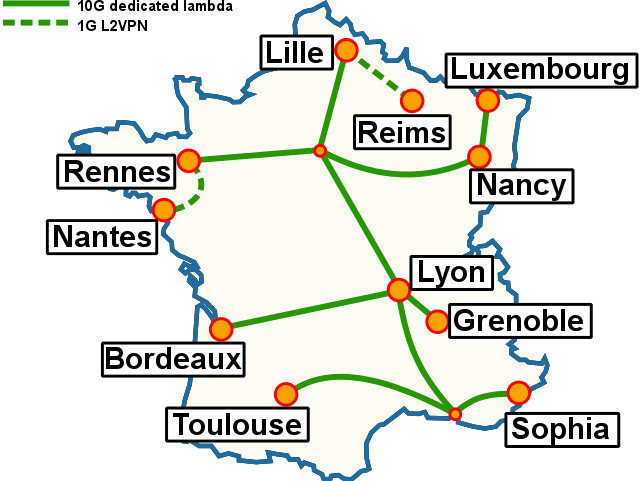
\includegraphics[scale=2]{./Figures/Renater5-g5k.jpg}
    \rule{35em}{0.5pt}
  \caption[Grid'5000 sites]{The sites of Grid'5000}
  \label{fig:Electron}
\end{figure}
It is very important with regard to the
experiments that inter-site communication and inter-node communication
are unrestricted and don't weigh any overhead on the
experiments. Thus, all communication can be done without any
constraints between sites. But
as for security, we have to take into account the following: if a
node is fully reconfigurable by the researcher, that means we
can't make any assumptions about the configuration of the security
mechanisms on an allocated node, thus, we have to assume that they are
unprotected. This is the reasoning behind the decision that sites
themselves (thus, of course, the nodes they are hosting) are not
directly connected to the Internet, making Grid'5000 an isolated
domain. This way, the sites are protected against DoS attacks.\\
It is possible to open restricted routes through the Internet to
external clusters, which provides the possibility of doing
multiplatform experiments.
\subsubsection{User view and data management}
As previously mentioned, communication is done with minimal
restrictions between Grid'5000 machines, meaning that authentication
procedures in such cases is also minimal: a user has a single account
across the whole platform. An LDAP directory is installed to provide
this in a reliable way. Every site runs an LDAP server. These servers
have the same root and there is a branch for every site. On a given
site, the local administrator has read-write access, as well as is
able to manage user accounts.\\
A user has access to all of the Grid'5000 sites and services
(monitoring tools, wiki, deployment, etc.). The user also has an
independent home directory at every site as well. Synchronization can
be done with any of the standard tools, such as \emph{rsync},
\emph{scp}, or \emph{sftp}. Data transfers to the outside world are
restricted - it can only be done via secure tools such as \emph{scp}
in order to prevent identity spoofing. Authentication is done via a
user-generated public key, in order to prevent brute-force attacks.
\subsubsection{Experiment scheduling}
At cluster level, the OAR\cite{xdghmmnr05} resource management system is
used to handle the scheduling of experiments and resource
allocation. Large-scale operations such as parallel task launching or
monitoring is handled by a specialized parallel launching tool,
Taktuk\cite{chr09}. Taktuk is a handy tool which can be used from the
console to, for example, perform a certain set of tasks on multiple
nodes.\\
A simple grid broker is handling resource management at grid
level, allowing co-allocation of nodes on multiple
clusters. Co-allocation is a very simple process for the user who,
after submitting an experiment needing several sets of nodes across
different clusters, receives an identifier from the broker which can
be used to retrieve all necessary information about the allocated
nodes.\\
Node reconfiguration, talked about in more detail below, co-operates
with the resource management system at certain points. Such a point is
that when a user submits an experiment that requires node
reconfiguration, the job submission is registered in a queue. Also, in
the prologue script that runs before the actual experiment, deployment
rights are given to the user which gives him/her the capability to
deploy system images on the allocated nodes. An epilogue script runs
after the experiment, revoking these rights. After the experiment is
finished, all of the allocated nodes are rebooted, deploying a default
environment, to provide a constant, unified system to run experiments
on that don't need node reconfiguration.
\subsubsection{Node reconfiguration}
Node reconfiguration on Grid'5000 is handled in a very user-friendly
way, using a tool called Kadeploy3\cite{jsn13}. For every user, a set
of default environments is available at start. After starting an
interactive job (that is, a job that requires node reconfiguration),
the user can deploy any of these environments by providing the chosen
image's name to Kadeploy3. Deployment usually takes only a few minutes
to complete - deployment time increases if we do the deployment on
more nodes. After this, the nodes are rebooted and the user can log
onto any of the nodes where an image was successfully deployed. When
logged in, the user can freely customize the environment: he/she can
install or remove software, modify configuration files, etc. - root
password is given to Grid'5000 users as well to provide more
possibilities. After reconfiguring the environment, the user has the
the possibility of saving the now customized image. This image
includes all software layers from OS to application levels, just as it
was for the default environments. The home directory is independent of
the image. After successfully saving an image, the user can deploy it
on the allocated nodes the same way he/she did for the default
images. This way, an environment tailored for the specific needs of
the user only needs to be created once, then it can be freely reused
on any other node on the site at a later time. When trying to port an
image created on one site to another site, there can be compatibility
issues due to inter-site differences. Modifications to the customized
image can be done with ease.
